\documentclass[a4paper]{jsarticle}
\usepackage[dvipdfmx]{graphicx}
\usepackage{amsmath}
\usepackage{bm}
\renewcommand{\thesection}{第\arabic{section}問}
\renewcommand{\thesubsection}{(\arabic{subsection})}
\renewcommand{\thesubsubsection}{(\alph{subsubsection})}
\begin{document}

\title{2022分野3}
\author{nakao}
\maketitle

\section{}
\subsection{}
式[2]において
$\frac{\partial v}{\partial t} = 0, i_f = 0$
として、
\begin{equation}
  \frac{\partial}{\partial x}
  \left(\frac{v^2}{2g} + h + z\right) = 0
\end{equation}
となる。

\subsection{}
気持ち悪いので
$i_0 = -\frac{\partial z}{\partial x}$
として進めます。出題ミス??
\subsubsection{}
エネルギー保存則は、
\begin{equation}
  \frac{\partial E_s}{\partial x} = i_0 - i_f
\end{equation}
と表される。等流のとき$h = h_0$で一定であるから
\begin{align}
  \frac{\partial E_s}{\partial x}
  &= \frac{\partial}{\partial x}
  \left(\frac{q^2}{2 g h_0^2} + h_0\right)
  = 0 \\
  i_f &= n^2 h_0^{-\frac{4}{3}} \left(\frac{q}{h_0}\right)^2
  = n^2 q^2 h_0^{-\frac{10}{3}}
\end{align}
となり、これらを式(2)に代入すると、
\begin{equation}
  h_0 = \left(\frac{n^2 q^2}{i_0}\right)^{\frac{3}{10}}
\end{equation}
が得られる。

\subsubsection{}
式(5)より
\begin{equation}
  \frac{\partial E_s}{\partial x}
  = i_0 - i_f
  = i_0 \left\{1 - \left(\frac{h_0}{h}\right)^{\frac{10}{3}}\right\}
\end{equation}
が成り立つから、
$h > h_0$のとき、$\frac{\partial E_s}{\partial x} > 0$であり、
また$h < h_0$のとき、$\frac{\partial E_s}{\partial x} < 0$となる。

\subsubsection{}
$h = h_0$で一定のとき、満たすべき条件は
\begin{equation}
  \mathrm{Fr}^2 = \frac{q^2}{g h_0^3} > 1
\end{equation}
であり、式[5]を代入して計算すると
\begin{equation}
  i_0 > n^2 q^{-\frac{2}{9}} g^{\frac{10}{9}}
\end{equation}
を得る。\par
以下、$\frac{\partial h}{\partial x} \neq 0$の場合を考える。
\begin{equation}
  \frac{\partial E_s}{\partial x}
  = \frac{\partial}{\partial x}
  \left(\frac{q^2}{2 g h^2} + h\right)
  = (1 - \mathrm{Fr}^2) \frac{\partial h}{\partial x}
\end{equation}
であり、式(2)とManningの式
$i_f = n^2 q^2 h_0^{-\frac{10}{3}}$
より、
\begin{equation}
  (1 - \mathrm{Fr}^2) \frac{\partial h}{\partial x}
  = i_0 - n^2 q^2 h_0^{-\frac{10}{3}}
\end{equation}
となる。したがって、満たすべき条件は、
\begin{equation}
  1 - \mathrm{Fr}^2 =
  \frac{i_0 - n^2 q^2 h_0^{-\frac{10}{3}}}{\frac{\partial h}{\partial x}} < 0
\end{equation}
と表せる。
$\frac{\partial h}{\partial x}$の符号に分けて記述すると、
\begin{equation}
  \begin{cases}
    i_0 < n^2 h^{-\frac{10}{3}} q^2
    & \left(\frac{\partial h}{\partial x} > 0\right) \\
    i_0 > n^2 h^{-\frac{10}{3}} q^2
    & \left(\frac{\partial h}{\partial x} < 0\right) \\
  \end{cases}
\end{equation}
である。

\subsubsection{}
式(6),(9)より、
\begin{equation}
  (1 - \mathrm{Fr}^2) 
  = i_0 \left\{1 - \left(\frac{h_0}{h}\right)^{\frac{10}{3}}\right\}
\end{equation}
が成り立つ。これより、
\begin{equation}
  \frac{\partial h}{\partial x}
  = i_0 \frac{1 - \left(\frac{h_0}{h}\right)^{\frac{10}{3}}}{1 - \mathrm{Fr}^2}
\end{equation}
である。ここで、射流の条件を常に満たすことを仮定しているため、
$1 - \mathrm{Fr}^2 < 0$である。\par
したがって、$h > h_0$のとき
$\frac{\partial h}{\partial x} < 0, \frac{\partial h}{\partial x} \xrightarrow{h \to h_0} 0$
が成り立つ。また、$h < h_0$のとき、
$\frac{\partial h}{\partial x} > 0, \frac{\partial h}{\partial x} \xrightarrow{h \to h_0} 0$
が成り立つ。

\subsection{}
式[3],[4]より
\begin{equation}
  \left(c - \frac{\mathrm{d} q}{\mathrm{d} h}\right)
  \frac{\partial h}{\partial x} = 0
\end{equation}
が成り立ち、波が進行するときに
$\frac{\partial h}{\partial x} \neq 0$
であるとすれば、
\begin{equation}
  c = \frac{\mathrm{d} q}{\mathrm{d} h}
  = \frac{\mathrm{d}}{\mathrm{d} h} (v h)
  = \frac{\mathrm{d}}{\mathrm{d} h} \left(n^{-1} h^{\frac{5}{3}} i_0^{\frac{1}{2}}\right)
  = \frac{5}{3} v
\end{equation}
である。

\subsection{}
Manningの式と式(16)より
\begin{equation}
  h = \left(v n i^{-\frac{1}{2}}\right)^{\frac{3}{2}}
  = \left(\frac{3}{5} c n i^{-\frac{1}{2}}\right)^{\frac{3}{2}}
\end{equation}
である。ここに、
$c = 1 \, \mathrm{km} / 200 \, \mathrm{s} = 5 \,\mathrm{m s^{-1}}$,
$n = 0.025 \, \mathrm{m^{-\frac{1}{3}} s}$,
$i_0 = 1/900$を代入すると、
$h = 3.375 \, \mathrm{m}$が得られる。

\subsection{}
\subsubsection{}
kinematic waveの運動方程式は、
$-i_0 + i_f = 0$であり、diffusion waveの運動方程式は、
$\frac{\partial h}{\partial x} - i_0 + i_f = 0$である。
それぞれにManningの式
$v = n^{-1} h^{\frac{2}{3}} i_0^{\frac{1}{2}}$
を代入すると、それぞれの流量は、
\begin{align}
  q_{kine} &= n^{-1} h^{\frac{5}{3}} i_0^{\frac{1}{2}} \\
  q_{diff} &= n^{-1} h^{\frac{5}{3}} \left(i_0^{\frac{1}{2}} - \frac{\partial h}{\partial x}\right)
\end{align}
と表される。したがって、水深-流量の関係の概略図は図1の通り。
diffusion waveでは、水深の勾配に応じて、kinematic waveからの流量がずれる。
\begin{figure}[htb]
  \centering
  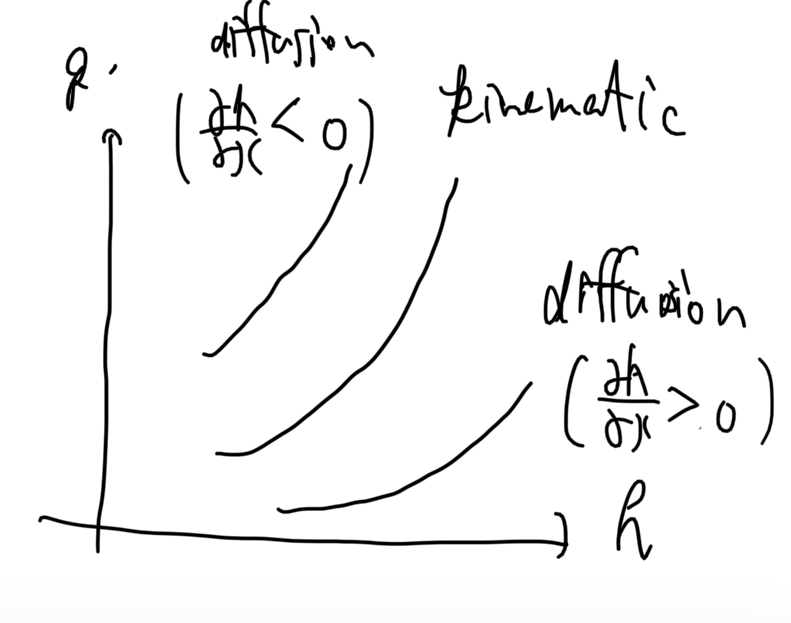
\includegraphics[width=0.3\hsize]{fig1.png}
  \caption{水深-流量の関係の概略図}
\end{figure}

\subsubsection{}
小河川における大河川との合流部など、下流側の水位が高くなっている場所。
下流側からの逆流により、流量のキャパシティが減少する。

\subsection{}
災害規模と被害規模の関係を推察することができるようになり、
防災の効果が検証しやすくなる。費用対効果の高い施策が行うための意思決定に役立つ。
市民はどのような災害に対して居住地域が大きな被害を受けるかを確認し、
自身がどのタイプの災害を恐れるべきか理解できる。

\section{}
\subsection{}
Manningの式より$n = v^{-1} R^{\frac{3}{2}} I^{\frac{1}{2}}$である。
ここで、$v$は断面平均流速、$R$は径深、$I$はエネルギー勾配である。
水路が幅広矩形断面であるから、$R$は水深$h$で近似できる。
$I$は水面の勾配で近似する。$v$は断面内複数点で流速を計測したときの平均値とする。

\subsection{}
\subsubsection{}
図2のように岸に垂直な方向に$d$だけ離して2つの観測点A,Bをとる。
波の進行方向に$x$軸をとる。
$d$は波長$L$に対して十分小さく、点A,Bにおける水深は共通であるとする。\par
\begin{figure}[htb]
  \centering
  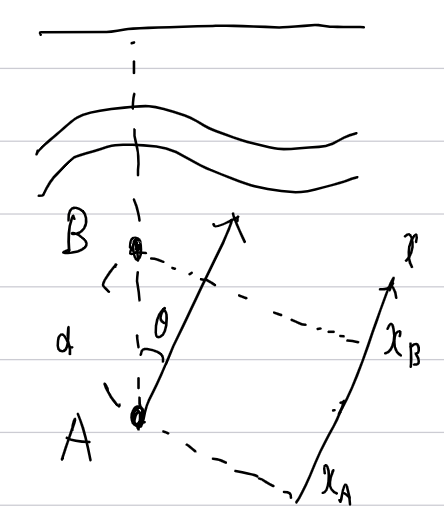
\includegraphics[width=0.3\hsize]{fig2.png}
  \caption{Survey plan Aの設定}
\end{figure}
微小振幅波理論により点A,Bの海底における水圧は、それぞれ
\begin{align}
  p_A(t) &= \rho g h + \frac{\rho g H}{2 \cosh k h} \cos (k x_A - \omega t) \\
  p_B(t) &= \rho g h + \frac{\rho g H}{2 \cosh k h} \cos (k x_B - \omega t) \\
\end{align}
と表せる。\par
$p_A(t), p_B(t)$の両方において、時間平均の値は$\rho g h$であり、ここから
$h = \frac{\overline{\rho (t)}}{\rho g}$が計算できる。\par
また$p_A(t),p_B(t)$の振動周期は波の周期$T$に等しく、\underline{この値が時系列から読み取れる。}\par
さらに、波の角振動数$\omega$は$\omega = \frac{2 \pi}{T}$で計算でき、分散関係式
$\omega^2 = g k \tanh k h$を考えれば$\omega, g, h$が既知だから
これを満たす波数$k$が定まる。\par
$p_A(t),p_B(t)$について、振動の振幅$\varDelta p$はどちらも
$\frac{\rho g H}{2 \cosh k h}$である。これより、
$H = \frac{2 \varDelta p \cosh k h}{\rho g}$が計算できる。\par
浅水係数$K_s$は、
\begin{equation}
  K_s = \sqrt{\frac{1}{2 n \tanh k h}},\quad
  n = \frac{1}{2} \left(1 + \frac{2 k h}{\sinh 2 k h}\right)
\end{equation}
と表され、$k,h$が既知であるからこの値が計算できる。
\underline{沖波波高$H_0$は
$H_0 = \frac{H}{K_s}$として計算できる。} \par
$p_B(t) = p_A(t - \frac{k (x_b - x_a)}{\omega})$と表せるため、
$p_A(t)$と$p_B(t)$の時間ずれを$\varDelta t$とすると、
$\varDelta t = \frac{k(x_b - x_a)}{\omega}$である。
$x_b - x_a = d \cos \theta$であるから、
$\cos \theta = \frac{\omega \varDelta t}{k d}$となり、
\underline{$\theta = \arccos \frac{\omega \varDelta t}{k d}$が計算できる。}

\subsubsection{}
図3のように任意の地点に観測点をとり、岸に平行な方向の流速$u_h(t)$と
岸に垂直な方向の流速$u_v(t)$を測定する。波の進行方向に$x$軸をとる。\par
\begin{figure}[htb]
  \centering
  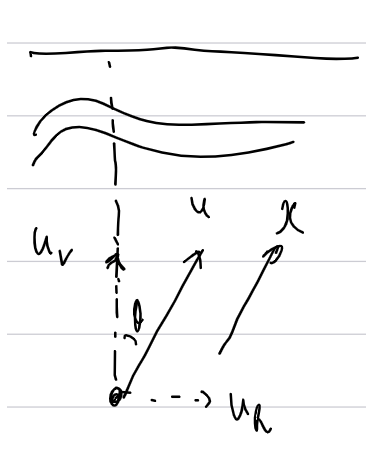
\includegraphics[width=0.3\hsize]{fig3.png}
  \caption{Survey plan Bの設定}
\end{figure}
微小振幅波理論によれば観測点において$x$軸方向の流速$u(t)$は
\begin{equation}
  u(t) = \frac{H \omega}{2 \sinh k h} \cos (k x - \omega t)
\end{equation}
と表される。$H$は波高、$\omega$は波の角振動数、$k$は波の波数である。
このとき、
$u_h(t) = u(t) \sin \theta, u_v(t) = u(t) \cos \theta$
より、
$\overline{u_h(t)} = \overline{u_(t)} \sin \theta, \overline{u_v(t)} = \overline{u_(t)} \cos \theta$
である。これより
\underline{$\theta = \arctan \frac{\overline{u_h(t)}}{\overline{u_v(t)}}$が計算できる。} \par
\underline{$u_h(t),u_v(t)$の振動の周期は波の周期$T$に一致}し、
$\omega = \frac{2 \pi}{T}$が計算できる。
これと分散関係式
$\omega^2 = g k \tanh k h$を考えれば、
$\omega, h$が既知だからこれを満たす$k$が定まる。\par
$u_h(t)$の振幅は$\frac{H \omega \sin \theta}{2 \sinh k h}$であり、
この値を$\varDelta u$とすると、$\omega, \theta, k, h$が既知であるから
$H = \frac{2 \varDelta u \sinh k h}{\omega \sin \theta}$が計算できる。
また、$k, h$が既知であるから、浅水係数$K_s$が式(23)から計算できる。\par
\underline{沖波波高$H_0$は
$H_0 = \frac{H}{K_s}$として計算できる。}

\subsection{}
任意の地点に観測点をとり、海底における岸に垂直な水平方向の流速と水圧を計測する。
入射波と反射波の波形をそれぞれ
\begin{equation}
  \eta_I = a_I \cos (kx - \omega t),\quad
  \eta_R = a_R \cos (kx + \omega t)
\end{equation}
とすると、微小振幅波理論によりそれぞれの水平方向流速は
\begin{equation}
  u_I = \frac{\omega}{\sinh k h} \eta_I,\quad
  u_R = \frac{\omega}{\sinh k h} \eta_R
\end{equation}
と表せる。これより、流速の観測値$u$について、
\begin{equation}
  u = u_I - u_R = \frac{\omega}{\sinh k h} (\eta_I - \eta_R)
\end{equation}
と表せる。\par
海底での水圧の観測値$p$は、
\begin{equation}
  p = \rho g h + \rho g (\eta_I + \eta_R)
\end{equation}
となる。ここで、$h$は水深である。$p$の時間平均について、
$\overline{p} = \rho g h$より、
$h = \frac{\overline{p}}{g h}$が計算できる。\par
また、
\begin{equation}
  \begin{aligned}
    \eta_I + \eta_R
    &= a_I (\cos k x \cos \omega t + \sin k x \sin \omega t)
    + a_R (\cos k x \cos \omega t - \sin k x \sin \omega t) \\
    &= (a_I + a_R) \cos k x \cos \omega t
    + (a_I - a_R) \sin k x \sin \omega t \\
    &= \sqrt{(a_I + a_R)^2 \cos^2 k x + (a_I - a_R)^2 \sin^2 k x} \cos (\omega t - \delta)
  \end{aligned}
\end{equation}
と表せることから、$\eta_I + \eta_R$の振動数は$\omega$である。
$p$の振動成分は$\rho g (\eta_I + \eta_R) \propto \eta_I + \eta_R$より、
$p$の振動数も$\omega$である。ここから$\omega$が決定できる。\par
さらに分散関係式$\omega^2 = g k \tanh k h$において
$\omega, h$が既知であるから、これを満たす波数$k$が定まる。\par
式(27),(28)より、
\begin{align}
  \eta_I &= \frac{1}{2} \left(\frac{p}{\rho g} - h + \frac{u \sinh k h}{\omega}\right) \\
  \eta_R &= \frac{1}{2} \left(\frac{p}{\rho g} - h - \frac{u \sinh k h}{\omega}\right)
\end{align}
が成り立つ。$h, \omega, k$が既知であるから、
$u, p$の観測から、その点における$\eta_I, \eta_R$の信号を推定することができる。
ここから反射率$K_R = \frac{\max \eta_I}{\max \eta_R}$が求められる。
\end{document}